\begin{center}
    \addcontentsline{toc}{section}{ГЛАВА 1. ЗАДАЧА РЭКАНСТРУКЦЫІ ПАВЕРХНІ}
    \section*{ГЛАВА 1. \\ Задача рэканструкцыі паверхні}
\end{center}

\addcontentsline{toc}{subsection}{1.1 Агульныя звесткі}
\subsection*{1.1 Агульныя звесткі}

У агульным выпадку задача рэканструкцыі паверхні фармулюецца наступным чынам:
неабходна рэканструяваць трохмерны аб'ект па мностве зробленых з розных ракурсаў
здымкаў. Задача досыць натуральная і калі чалавеку дастаткова кінуць
позірк на аб'ект, каб уявіць ягоную трохмерную структуру, алгарытмічна задача
ўсё яшчэ застаецца не цалкам вырашанай, патрабуе досыць вялікіх вылічальных магутнасцяў
і не працуе ўніверсальна добра для любых асяроддзяў і любых умоваў здымак.

Задача рэканструкцыі можа таксама фармулявацца для іншых тыпаў уваходных дадзеных:
апроч камеры ўваходнымі дадзенымі для задачы могуць быць
дадзеныя з іншых датчыкаў, такіх як акселерометр, гіраскоп ці GPS-датчык;
замест манакулярнай камеры можа прымяняцца RGB-D (вяртае дадатковы слой глыбіняў)
ці стэрэа камера, якая ўяўляе сабой дзве RGB камеры
і ў пэўным сэнсе імітуе бінакулярны чалавечы зрок.

У залежнасці ад таго, якія выходныя дадзеныя нас цікавяць, алгарытм можа будаваць
воблака кропак рознай шчыльнасці альбо будаваць шчыльную тэкстураваную мадэль
максімальна падобную на рэальны трохмерны аб'ект. Розныя патрабаванні да выходных
дадзеных патрабуюць адрозных алгарытмічных рашэнняў і наяўнасці розных вылічальных магутнасцяў.

Варта дадаць, што даследаванні ў гэтай галіне кампутарнага зроку развіваюцца
таксама праз удасканаленне апаратнага забеспячэння: падыходы, якія некалькі год
таму былі практычна нерэалізуемымі, з развіццём тэхналогіяў даюць ім новае жыццё.

\addcontentsline{toc}{subsection}{1.2 Сферы прымянення}
\subsection*{1.2 Сферы прымянення}

Цікавасць задачы рэканструкцыі таксама ў запатрабаванні атрымання рашэння ў абсалютна розных сферах
жыцця, у кожнай на сваімі асаблівасцямі.

БПЛА выкарыстоўваюцца надзвычайнымі службамі для ацэнкі наступстваў прыродных катастроф,
у сельскай гаспадарцы, дарожнымі службамі. Патрабаванні да хуткасці працы алгарытмаў рэканструкцыі
натуральныя - хуткасць працы ў некаторых галінах жыцця крытычная і разбор вялікіх аб'ёмаў
неапрацаваных дадзеных чалавекам можа быць немагчымы. Патрабаванні да працы алгарытмаў
рэканструкцыі ў рэальным часе ў большасці выпадкаў з'яўляюцца пры навігацыі і
аўтаномным руху, у такім выпадку шчыльная рэканструкцыя можа быць залішняй і
разрэджаная мадэль у выглядзе воблака кропак цалкам задаволіць патрабаванні.

\addcontentsline{toc}{subsection}{1.3 Адрозненні ў тыпах камер}
\subsection*{1.3 Адрозненні ў тыпах камер}

Неглядзячы на цікавыя магчымасці такіх датчыкаў, як акселерометр, гіраскоп альбо
лазер вымярэння адлегласці, яны не заўсёды даступныя і не даюць універсальна добрых
вынікаў у любых умовах. Далей мы будзем весці гутарку пра розныя тыпы камер і
больш за ўсё - пра манакулярную, як найбольш універсальную, распаўсюджаную і простую
ў эксплуатацыі.

\vspace{5mm}
{\bf Манакулярная RGB камера}

Самымі распаўсюджанымі з'яўляюцца манакулярныя камеры - камеры, якія прысутнічаюць
у смартфонах, ужываюцца ў быце і з якімі мы ўсе выдатна знаёмыя.
Манакулярныя камеры ў сваю чаргу таксама бываюць розных тыпаў,
але на практыцы мы часцей за ўсё працуем з праэктыўнымі (projective, pinhole) камерамі.

Праецыраванне трохмерных кропак у гэтым выпадку можа быць апісанае наступнай формулай:

\begin{equation}
  x = PX
\end{equation}

дзе $P$ - матрыца, якая здзяйсняе пераўтварэнне, $X, x$ - вектары, якія адпавядаюць
трохмернай і двухмернай кропцы адпаведна, запісаныя ў аднародных каардынатах.
У сваю чаргу матрыцу $P$ можна прадставіць як:

\begin{equation}
  P = K[R|t]
\end{equation}

дзе $K$ - вектар унутраных параметраў камеры, $R$ - матрыца павароту, $t$ - вектар
зрушэння камеры ў прасторы ў сусветных каардынатах. Гэтыя параметры задаюць праектыўную
камеру, якая здзяйсняе праекцыю кропкі прасторы на матрыцу камеры. Унутраныя параметры могуць
задавацца разнастайным чынам, распаўсюджанымі прыкладамі могуць быць матрыцы:

\begin{equation}
  K = \begin{bmatrix}
    f & 0 & p_x \\[0.3em]
    0 & f & p_y \\[0.3em]
    0 & 0 & 1
  \end{bmatrix},
  \hspace{5mm}
  K = \begin{bmatrix}
    \alpha_x & 0 & p_x \\[0.3em]
    0 & \alpha_y & p_y \\[0.3em]
    0 & 0 & 1
  \end{bmatrix}
\end{equation}

дзе $f$ - фокусная адлегласць, $\alpha_x$, $\alpha_y$ - фокусная адлегласць уздоўж восяў
(для выпадкаў, калі не супадае), $p_x$, $p_y$ - зрушэнні цэнтру праекцыі адносна цэнтра матрыцы.
Іншымі параметрамі камеры могуць быць радыяльныя скажэнні $k_1, k_2$, якія ўзнікаюць з-за неідэальнасці
лінзаў у камерах.

Унутраныя параметры камеры заўжды вядомыя загадзя альбо праз дакументацыю да прылады ад
вытворца, альбо праз каліброўку: каліброўка можа выяўляць хібы, дапушчаныя вытворцам.
Каліброўка дае добрыя значэнні ўнутраных параметраў
камеры, таму яны рэдка выкарыстоўваюцца ў якасці аптымізуемых параметраў.

Варта зазначыць, што адной з найбольшых перавагаў і, адначасова, адной з найбольшых
перашкодаў у працы ў манакулярнымі камерамі з'яўляецца неадназначнасць працы з масштабам.
Праблема ў тым, што масштаб не можа быць высветлены праз перасоўванні ў прасторы і
змяненні ў вуглах агляду, што з'яўляецца крыніцай мноства памылак. Разам з тым,
перавага неадназначнасці масштабу ва ўніверсальнасці: алгарытм будзе працаваць
з аднолькавымі вынікамі як у маленькіх закрытых памяшканнях, так і на вялікіх
адкрытых прасторах.

\vspace{5mm}
{\bf Стэрэа RGB камера}

Для стэрэа камеры ўласцівая наяўнасць двух ці больш аб'ектываў, кожны з якіх
стварае кадры незалежна ад іншых. Гэта дазваляе сімуляваць бінакулярны зрок чалавека
і атрымліваць трохмерныя аб'екты са значна меншымі вылічальнымі выдаткамі.
Кожны з аб'ектываў стэрэакамеры працуе як асобная манакулярная камера, плыні кадраў
з розных аб'ктываў даюць магчымасць праз пошук асаблівых кропак і геаметрыю
размясціць кропкі ў трохмернай прасторы.

Трэба дадаць, што стэрэа камера заўжды наладжаная на працу з пэўным спектрам адлегласцяў:
камера, якая працуе добра ў маленькіх закрытых прасторах не дасць такіх жа вынікаў,
калі прастора будзе змасштабаваная ў дзясяткі разоў. Такім чынам, стэрэа камеры не
ўласцівая такая ж універсальнасць у сферах прымянення, як для манакулярнай.

\vspace{5mm}
{\bf RGB-D камера}

RGB-D камера, як і стэрэа, з'яўляецца шматканальнай: разам з RGB каналам, які
вяртае звыклыя нашаму воку каляровыя выявы, існуе дадатковы канал, які для кожнага
здымка вяртае гэтак званую мапу глыбіняў. Прыклад вяртаемых дадзеных - на малюнку
\ref{fig:rgbd-example}.

На практыцы RGB-D камеры не заўсёды працуюць так добра, як нам хацелася б:
справа ў абмежаванасці спектра, у якім фармуюцца значэнні глыбіняў. Мапа глыбіняў,
атрыманая апаратным спосабам, часцей за ўсё выкарыстоўваецца для папярэдняй ініцыялізацыі
і для паслядоўнай аптымізацыяй алгарытмічнымі спосабамі.

Прыкладамі RGB-D камер з'яўляюцца Kinect для Xbox 360 альбо Intel RealSense камеры.

\begin{figure}[H]
\centering
\begin{subfigure}{.5\textwidth}
  \centering
  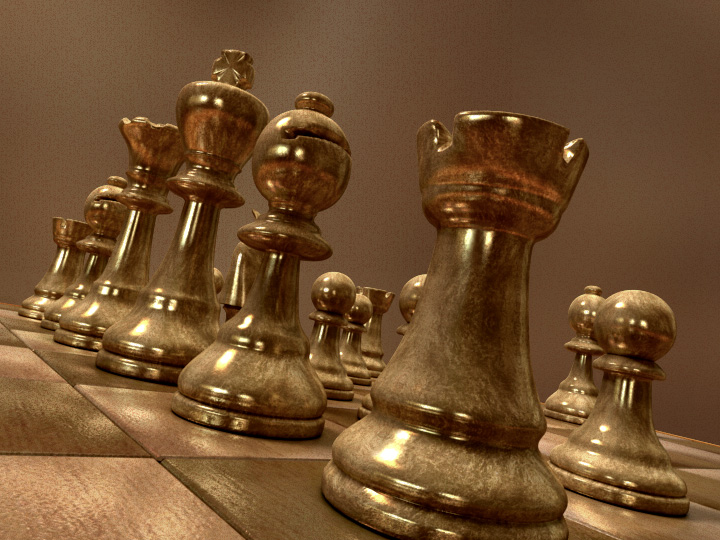
\includegraphics[width=.95\linewidth]{chess_rgb.jpg}
\end{subfigure}%
\begin{subfigure}{.5\textwidth}
  \centering
  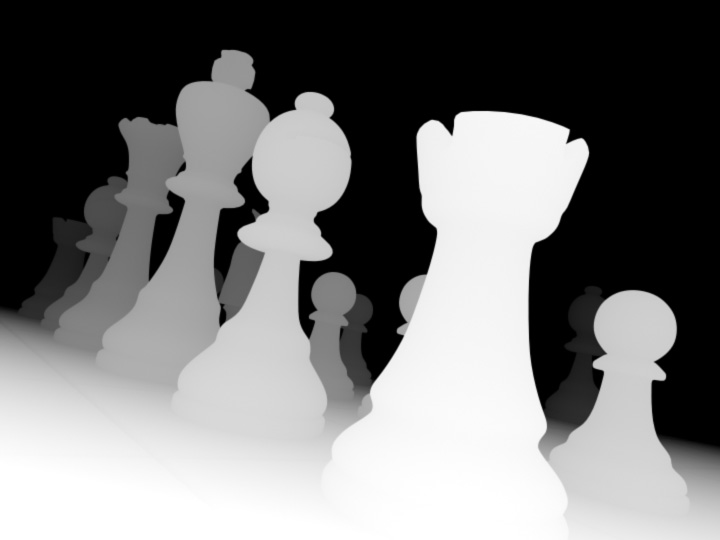
\includegraphics[width=.95\linewidth]{chess_d.jpg}
\end{subfigure}
\captionsetup{labelformat=empty}
\caption{Малюнак \arabic{figure}: здымкі з RGB-D камеры}
\label{fig:rgbd-example}
\end{figure}

\addcontentsline{toc}{subsection}{1.4 Рэканструкцыя паверхні афлайн}
\subsection*{1.4 Рэканструкцыя паверхні афлайн}

\begin{figure}[H]
  \centering
  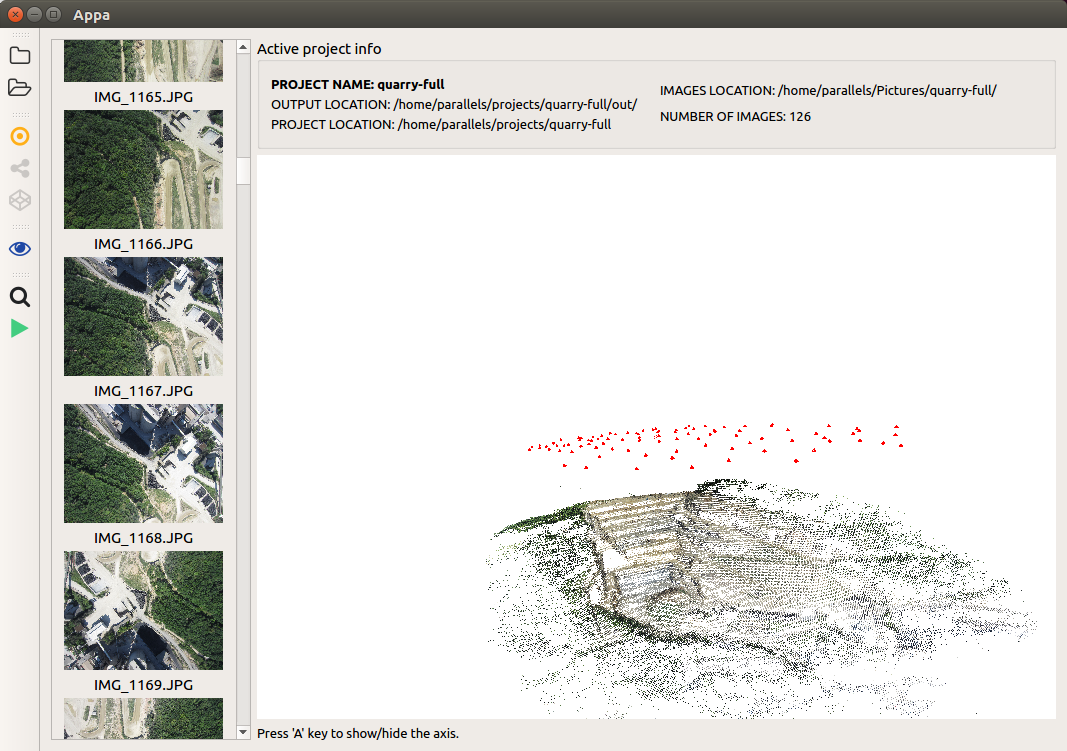
\includegraphics[width=.9\textwidth]{appa}
  \captionsetup{labelformat=empty}
  \caption{Малюнак \arabic{figure}: праграма рэканструкцыі паверхняў Appa}
  \label{fig:appa}
\end{figure}

Праект афлайн пабудовы трохмернай паверхні па здымках з манакулярнай камеры можа
ўключаць ў сябе наступныя этапы:

\begin{enumerate}
  \item Пошук і апісанне асаблівых кропак на выяве. Дасягаецца праз прымяненне
  такіх алгарытмаў і тыпаў дэскрыптараў, як SIFT \cite{sift-paper},
  SURF \cite{surf-paper}, ORB \cite{orb-paper} і іншых.
  \item Пошук адпаведнасцяў паміж двухмернымі кропкамі з мэтай знайсці
  кропкі, якія адпавядаюць адным і тым жа кропкам трохмернай прасторы (працэс \textit{matching}).
  \item Прымяненне эпіпалярнай геаметрыі для пошуку пазіцыяў трохмерных кропак
  і пазіцыяў камераў у прасторы. Унутраныя параметры камеры могуць як быць вядомымі
  і замацаванымі, так і ўдзельнічаць у наступнай аптымізацыі.
  \item Запуск алгарытмаў пучковай аптымізацыі (\textit{Bundle Adjustment}) для
  ўдасканалення пазіцый кропак, пазіцый і паваротаў камер у прасторы, унутраных
  параметраў камер (калі не вядомыя).
  \item Ушчыльненне, нанясення тэкстураў ды іншыя пераўтварэнні для перахода ад
  разрэджанага воблака кропак да шчыльных трохмерных мадэляў.
\end{enumerate}

Прыкладам бібліятэкі для пабудовы трохмернай мадэлі па такой схеме можа выступіць TheiaSfm
(\cite{theia-sfm}), праграмным сродкам для візуалізацыі працэса - распрацаваная мной
раней у рамках курсавой працы праграма \textit{Appa}, працэс працы якой можна
назіраць на здымку \ref{fig:appa}.

\newpage
